%%%%%%%%%%%%%%%%%%%%%%%%%%%%%%%%%%%%%%%%%%%%%%%%%%%%%%%%%%%%%%%%%%%%%%%%%
% SJCIEE manuscript guide/template
% version 1.1, May 27, 2022. by T. Ueta
%%%%%%%%%%%%%%%%%%%%%%%%%%%%%%%%%%%%%%%%%%%%%%%%%%%%%%%%%%%%%%%%%%%%%%%%%
\documentclass[10pt,twocolumn]{jsarticle}            % for platex 
%\documentclass[10pt,twocolumn]{ltjsarticle}         % for lualatex 
\usepackage[top=30mm, bottom=25mm, left=18mm, right=18mm]{geometry}
\usepackage[bookmarks=false, colorlinks=true, 
	dvipdfmx,                        % comment this line out for lualatex 
	linkcolor=black, urlcolor=black, citecolor=black ]{hyperref}
\usepackage{newtxtext,newtxmath}
\usepackage{wrapfig}
\usepackage[dvipdfmx]{graphicx,xcolor}               % for platex
%\usepackage{graphicx,xcolor}                        % for lualatex 
\usepackage{secdot}
\usepackage{float}

\sectiondot{subsection}
\columnsep=12pt \columnseprule=0pt \jot=0pt
\topsep=0pt \parskip=0pt \parindent=12pt
\floatsep=10pt \textfloatsep=10pt \intextsep=10pt
\setlength{\abovedisplayskip}{10pt plus 5pt}
\setlength{\belowdisplayskip}{8pt plus 5pt}
\renewcommand{\textfraction}{0.1}
\renewcommand{\floatpagefraction}{0.1}
\renewcommand{\topfraction}{1.0}
\renewcommand{\baselinestretch}{0.9}
\makeatletter
\def\section{\@startsection {section}{1}{\z@}%
{1ex plus 0.3ex minus .2ex}{0.2ex plus .1ex}{\large\bfseries}}
\def\subsection{\@startsection{subsection}{2}{\z@}%
{0.7ex plus 0.3ex minus .2ex}{0.2ex plus .1ex}{\normalsize\bfseries}}
\def\subsubsection{\@startsection{subsubsection}{3}{\z@}%
{0.4ex plus 0.2ex minus .2ex}{0.2ex plus .2ex}{\normalsize}}
\renewenvironment{thebibliography}[1]{%
	\subsection*{\refname}\@mkboth{\refname}{\refname}%
	\list{\@biblabel{\@arabic\c@enumiv}}%
		{\settowidth\labelwidth{\@biblabel{#1}}%
		\leftmargin\labelwidth \advance\leftmargin\labelsep
		\setlength\baselineskip{13pt} \setlength\itemsep{0pt}
		\@openbib@code \usecounter{enumiv}%
		\let\p@enumiv\@empty \renewcommand\theenumiv{\@arabic\c@enumiv}}%
	\sloppy \clubpenalty4000 \@clubpenalty\clubpenalty
\widowpenalty4000 \sfcode`\.\@m}
{\def\@noitemerr {\@latex@warning{Empty `thebibliography' environment}}%
\endlist}
\makeatother
\pagestyle{empty}
%%%%%%%%%%%%%%%%%%%%%%%%%%%%%%%%%%%%%%%%%%%%%%%%%%%%%%%%%%%%%%%%%%%%%%%%%
% Please edit below
%%%%%%%%%%%%%%%%%%%%%%%%%%%%%%%%%%%%%%%%%%%%%%%%%%%%%%%%%%%%%%%%%%%%%%%%%
\begin{document}

\twocolumn[
\begin{center}
{\Large 
% 講演番号刷り入れ用余白を作るために\rule で空白を挿入しています.
% 刷り上がりを見ながら50mm * 45mm の空白を確保してください.
\rule{0mm}{0mm}ゲノム選抜のための双曲埋め込みの検討\\
Exploring Hyperbolic Embedding for Genomic Selection\\
}
\vspace*{3pt} 
{ \large
\begin{tabular}{ccccc}
森 樹伸${}^1$ & 木脇 太一${}^1$ & 小林 栄治${}^2$ & 大江 美香${}^2$ & 荒川 愛作${}^2$ \\ 
S. Mori${}^1$ & T. Kiwaki${}^1$ & E. Kobayashi${}^2$ & M. Ooe${}^2$ & A. Arakawa${}^2$ \\
\end{tabular}\\
\begin{tabular}{cccc}
近森 太志${}^3$ & 濱田 和希${}^3$ & 山口 亜利沙${}^1$ & 松川 和嗣${}^1$\\
T. Chikamori${}^3$ & K. Hamada${}^3$& A. Yamaguchi${}^1$& K. Matukawa${}^1$\\
\end{tabular}\\
(高知大学${}^1$, 農研機構${}^2$, 高知県畜産試験場${}^3$)
}
\end{center}
\vspace*{12pt} 
]

\section{背景}
近年,畜産分野では,ゲノム情報を用いた育種,すなわちゲノム選抜(Genomic Selection, GS)が盛んに行われている.
GSでは,従来の線形モデルでは捉えきれない非線形情報を活用するために,
機械学習の応用が注目されているが,
ゲノムデータ特有の高次元・小サンプル問題に起因する過学習が課題となっている\cite{GS}.
このため,次元削減や特徴量選択などの前処理が重要な役割を果たす.

そこで本研究では,ゲノムデータが持つ潜在的な階層構造に着目し,
階層構造の表現に優れる双曲空間への埋め込みを適用することで,
データを従来よりも低次元で表現し,
前述の問題の緩和を目指す.
なお,本稿では埋め込み手法の一つ HypHC\cite{hypHC}の実装結果について報告する.

\section{双曲埋め込み}
\subsection{双曲空間}
双曲空間は,一定の負の曲率をもつ非ユークリッド空間であり,
半径の増加に伴い体積が指数的に増加する特性を持つ.
これにより,階層が深まるにつれてノード数が指数的に増加する木構造(階層構造の一種)を自然に表現できるため,
階層構造の表現に優れているとされる.

双曲空間を表現するモデルはいくつか存在する.
例えば,Poincaré ball モデルは $\mathbb{B}^n=\{x\in\mathbb{R}^n\mid\|x\|<1\}$ と定義され,
単位球内で双曲空間を表現する.

\subsection{HypHC}
HypHCは,双曲空間(Poincaré ball モデル)上で
階層クラスタリング(Hierarchical Clustering, HC)的にデータを表現するための埋め込み手法である\cite{hypHC}.
HCは類似度に基づき,集団の構造を二分木で可視化する手法で,
類似度の高いペアは木の深部で,類似度の低いペアは根近くで結合するという方針を持つ.
この方針の木全体における達成度を評価する指標として,Dasguptaのコスト関数がある.
HypHCは,埋め込みから再構築される二分木に関してDasguptaのコストを最小化するように埋め込みを行う.

\section{土佐あかうしのSNPデータ}
本研究では,土佐あかうしを対象とし,GSで広く用いられる
一塩基多型(Single Nucleotide Polymorphism, SNP)データ(669 頭 $\times$ 58,995 SNP)を使用する.
埋め込み手法はHypHCを選択し,非類似度としてユークリッド距離を用いた.

\section{結果}
\begin{wrapfigure}[11]{l}{40mm}
\vspace{-0.3ex} % ← 図全体の位置を詰める(上)
\setlength{\abovecaptionskip}{-10pt}
\centering
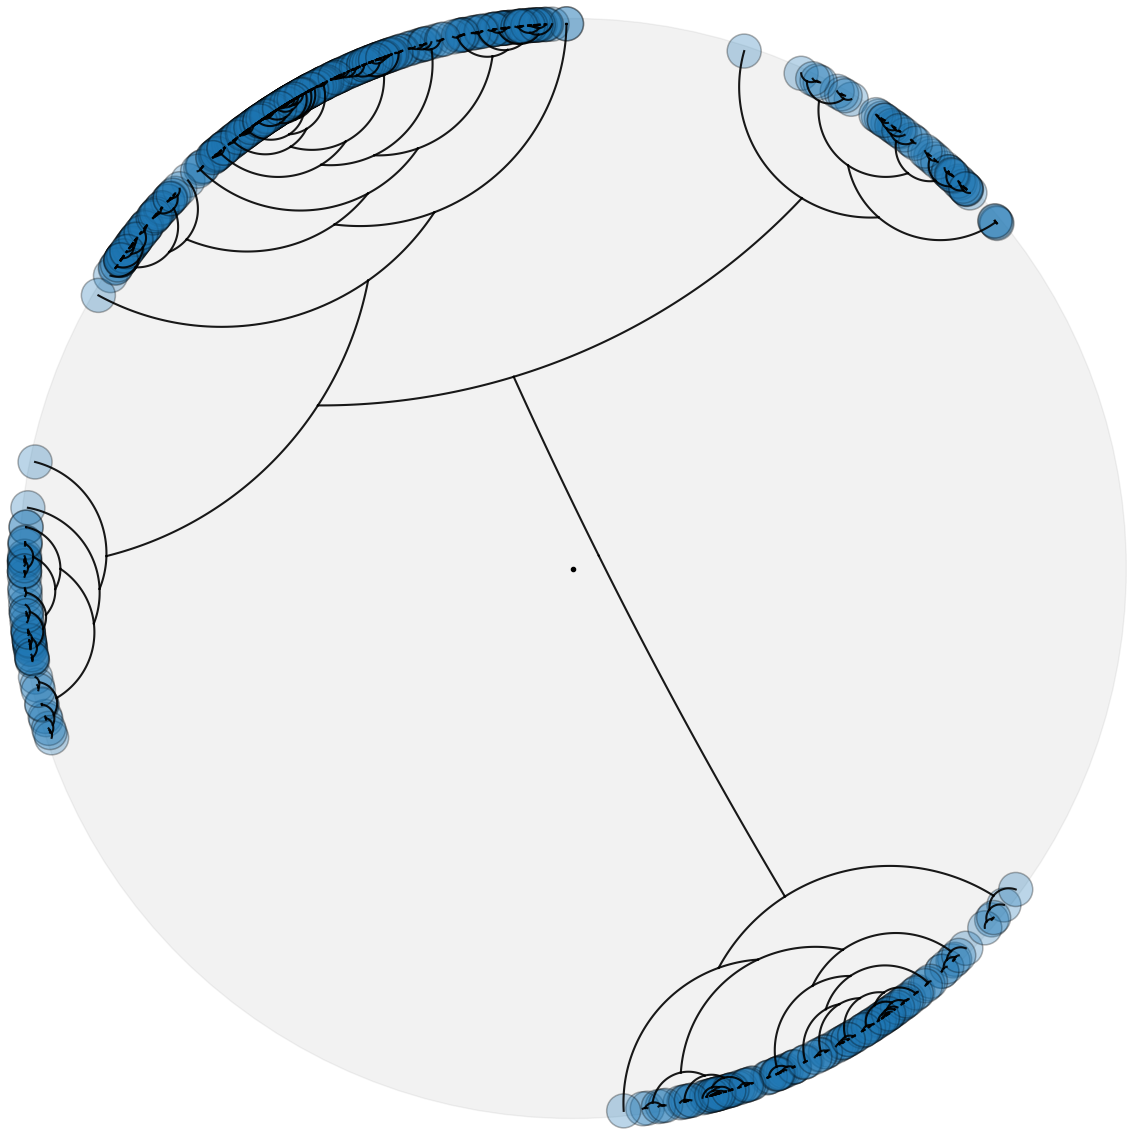
\includegraphics[width=43mm]{fig/SJCIEE_1.png}
\caption{HypHC (2 次元) の結果}
\label{fig:Embedding result}
\end{wrapfigure}
図\ref{fig:Embedding result}に 2次元双曲空間への埋め込みの結果を示す.
灰色の円はPoincaré ball モデル,青点は埋め込まれたデータ,実線は再構築された木を表す.
木は閾値 0.6 で 4 クラスタに分割され,図\ref{fig:Embedding result}でも定性的に確認できる.

表\ref{tab:d cost}に再構築された木のコストと,
HC の複数の結合方法(Ward,single,average,complete)の中で最小のコストとなった Ward法の結果を示す.
なお,埋め込み先の次元を増やすとコストはさらに改善したが,
50 次元以上では改善が見られなかった.


\begin{table}[H]
	\vspace{-0.3\baselineskip} % 表の上を詰めたい場合
	\centering
	\caption{Dasguptaのコストの比較}
	\label{tab:d cost}
	\begin{tabular}{|c|c|}
			\hline
			 & Dasgupta's cost ($\times 10^{10}$)  \\
			\hline
			HypHC (2 次元) & $-5.87$ \\
			HypHC (50 次元) & $-5.91$  \\
			\hline
			HC (Ward 法) & $-5.75$  \\
			\hline
	\end{tabular}
	\vspace{-0.3\baselineskip} % 表の下を詰めたい場合
\end{table}

\section{考察・展望}
図\ref{fig:Embedding result}で 4 クラスタが見られたが,
これが何を意味するかについては,
血統情報等との関係を調べ明らかにする必要がある.
また,50 次元でコストの改善が収束したことから,
HypHC では,50次元でデータを十分に表現できていると考えられる.
いずれにせよ,埋め込みの良し悪しは,
GSにおける予測精度で評価するべきであり,今後の課題とする.

\begin{thebibliography}{9}
 \bibitem{GS} 
Chafai et. al., ``A review of machine learning  models applied to genomic  prediction in animal breeding,''
 \textsl{Front. Genet.}, 14, article 1150596, 2023.
%
\bibitem{hypHC} 
Chami et. al., ``From Trees to Continuous Embeddings and Back:  Hyperbolic Hierarchical Clustering,''
\textsl{NeurIPS}, 33, pp.~15065-15076, 2020.
%
% \bibitem{web}
% 電気・電子・情報関係学会四国支部連合大会, 
% \url{https://sjciee.org} (2021年5月15日 参照)
\end{thebibliography}

\end{document}
